\section{Objectives of the analysis}
Here is an alloy specification of the system described in the RASD:

\section{Alloy Code}
\lstinputlisting[language=alloy]{Alloy/Alloy.als}


\section{Results}
\begin{figure}[H]
    \begin{center}
        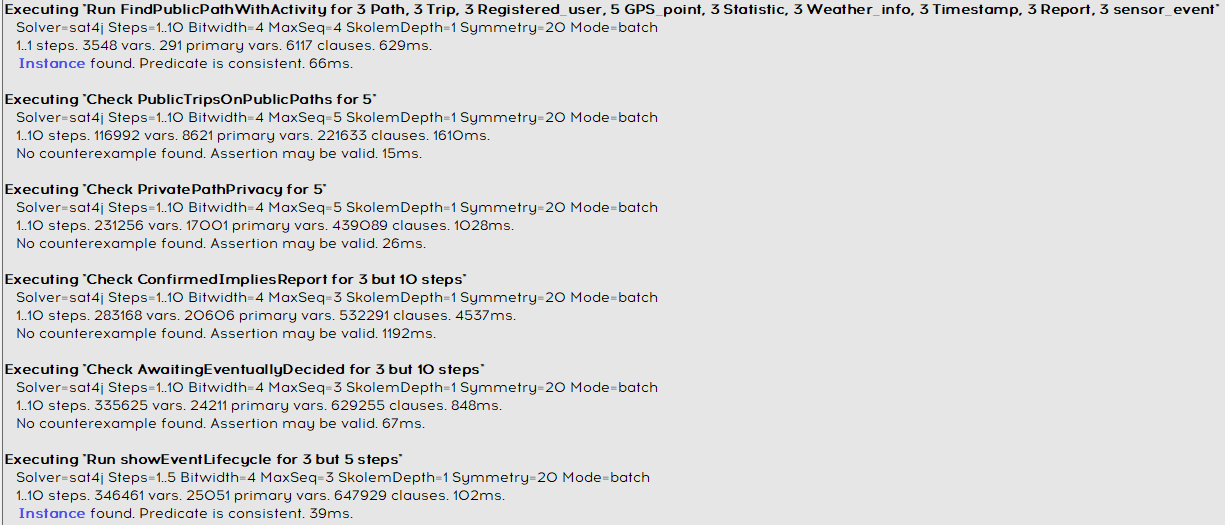
\includegraphics[width=1\linewidth]{RASD/LaTeXCode/Alloy/Formal analysis results.png}
        \caption{Formal analysis results.}
        \label{fig:Formal analysis results}%
    \end{center}
\end{figure}

\begin{figure}[H]
    \begin{center}
        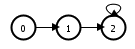
\includegraphics[width=0.3\linewidth]{RASD/LaTeXCode/Alloy/Alloy Sequence of states.png}
        \caption{Sequence of states.}
        \label{fig:Alloy Sequence of states}%
    \end{center}
\end{figure}

\subsection{States 0}

\begin{figure}[H]
    \begin{center}
        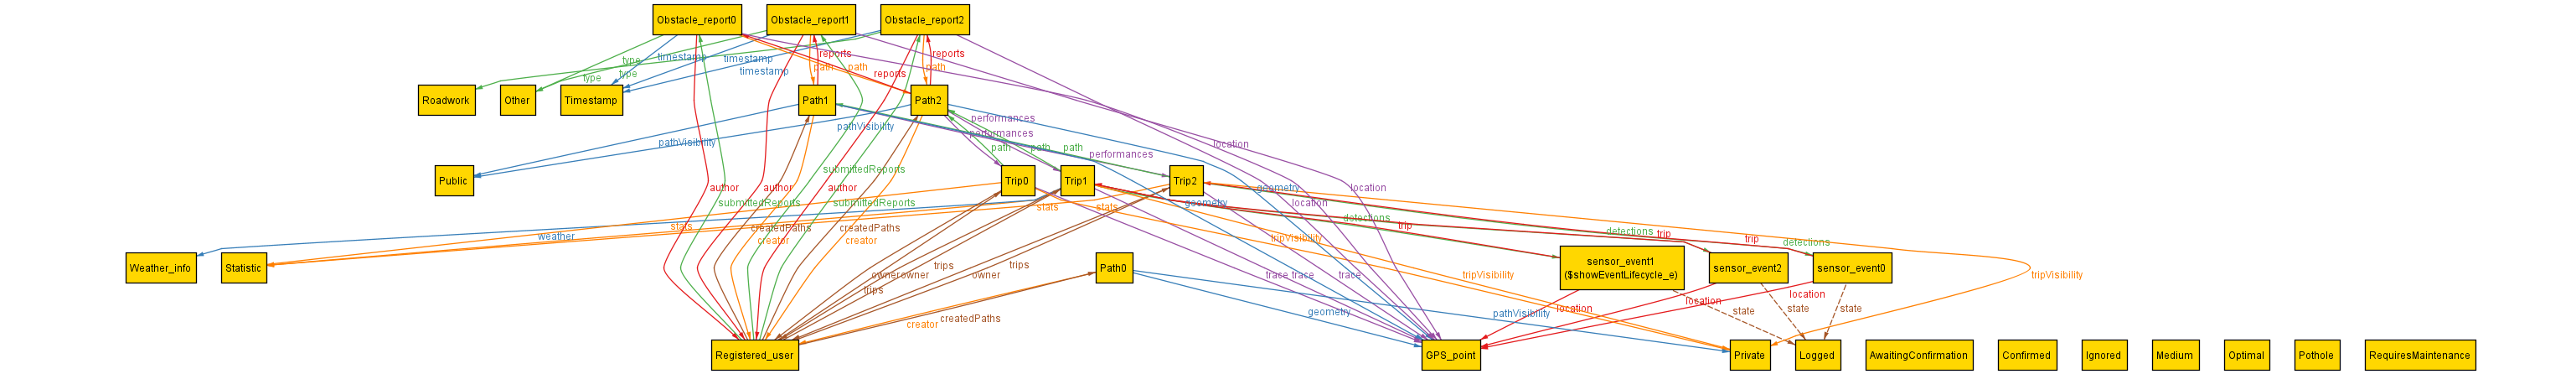
\includegraphics[angle=90,width=0.25\linewidth]{RASD/LaTeXCode/Alloy/State 0 Relational Graph.png}
        \caption{State 0 Relational Graph.}
        \label{fig:State 0 Relational Graph}%
    \end{center}
\end{figure}

\begin{figure}[H]
    \begin{center}
        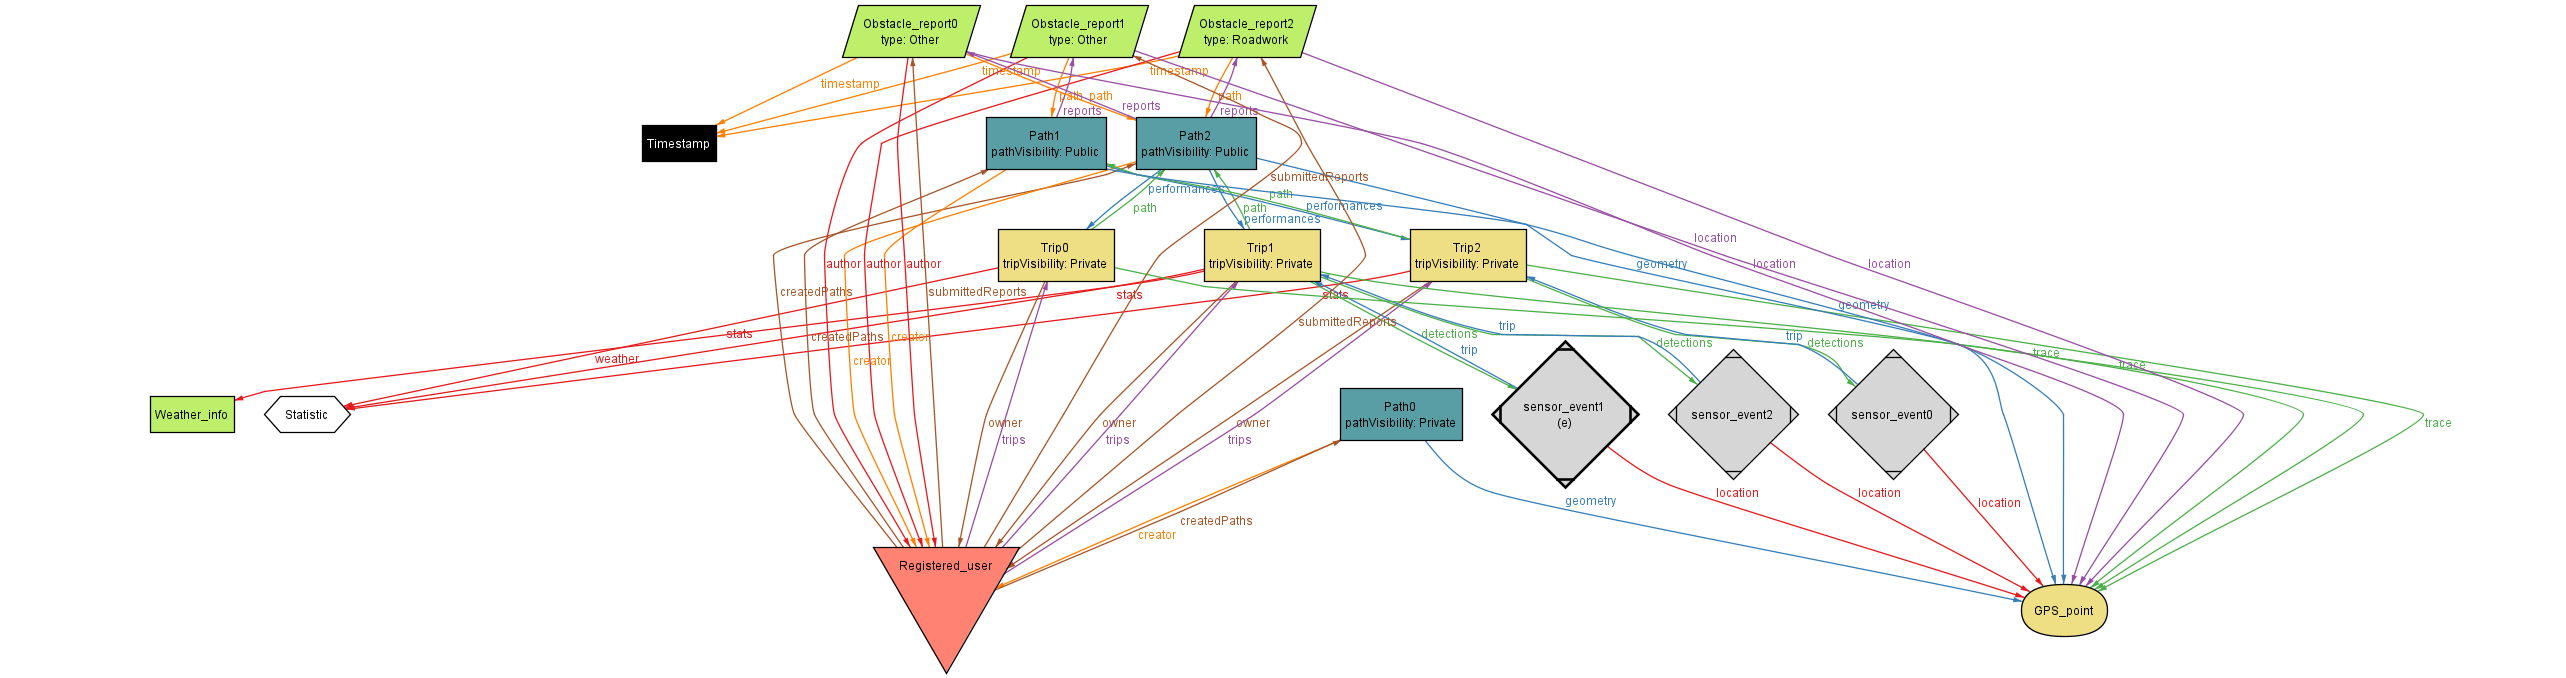
\includegraphics[width=1\linewidth]{RASD/LaTeXCode/Alloy/State 0 Projected View.png}
        \caption{State 0 Projected View}
        \label{fig:State 0 Projected View}%
    \end{center}
\end{figure}

\subsection{States 1}

\begin{figure}[H]
    \begin{center}
        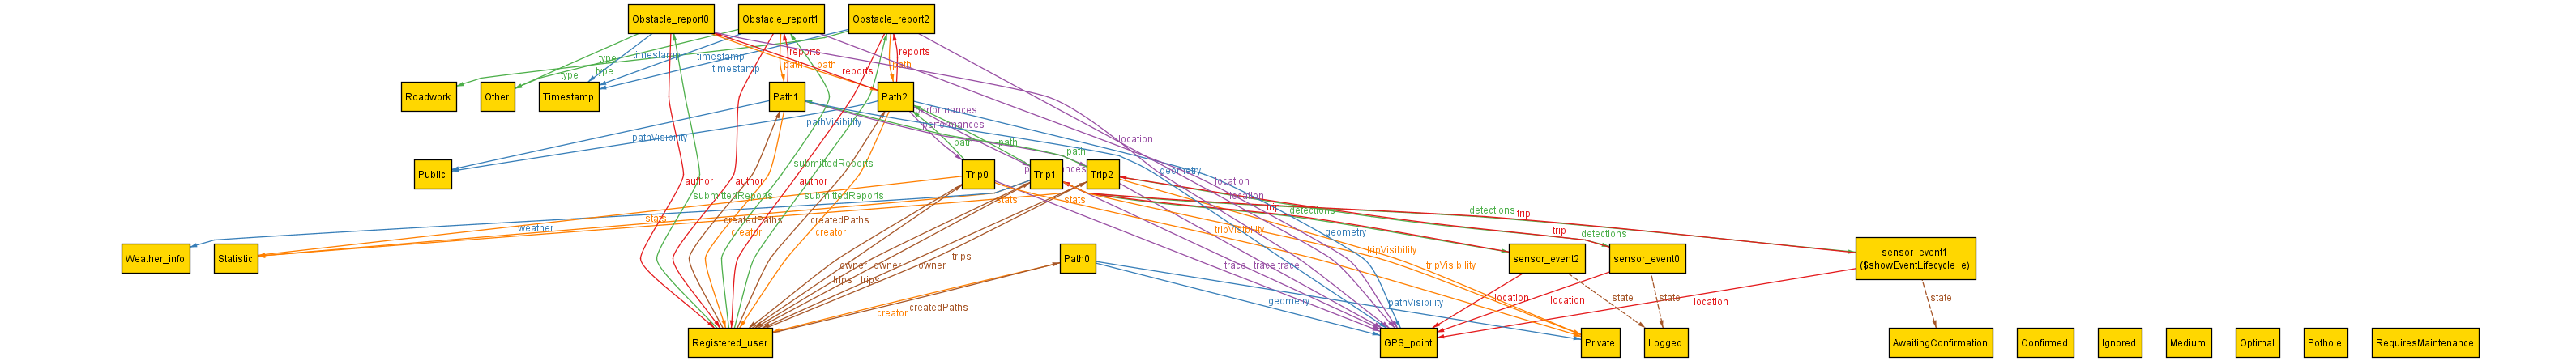
\includegraphics[angle=90,width=0.25\linewidth]{RASD/LaTeXCode/Alloy/State 1 Relational Graph.png}
        \caption{State 1 Relational Graph.}
        \label{fig:State 1 Relational Graph}%
    \end{center}
\end{figure}

\begin{figure}[H]
    \begin{center}
        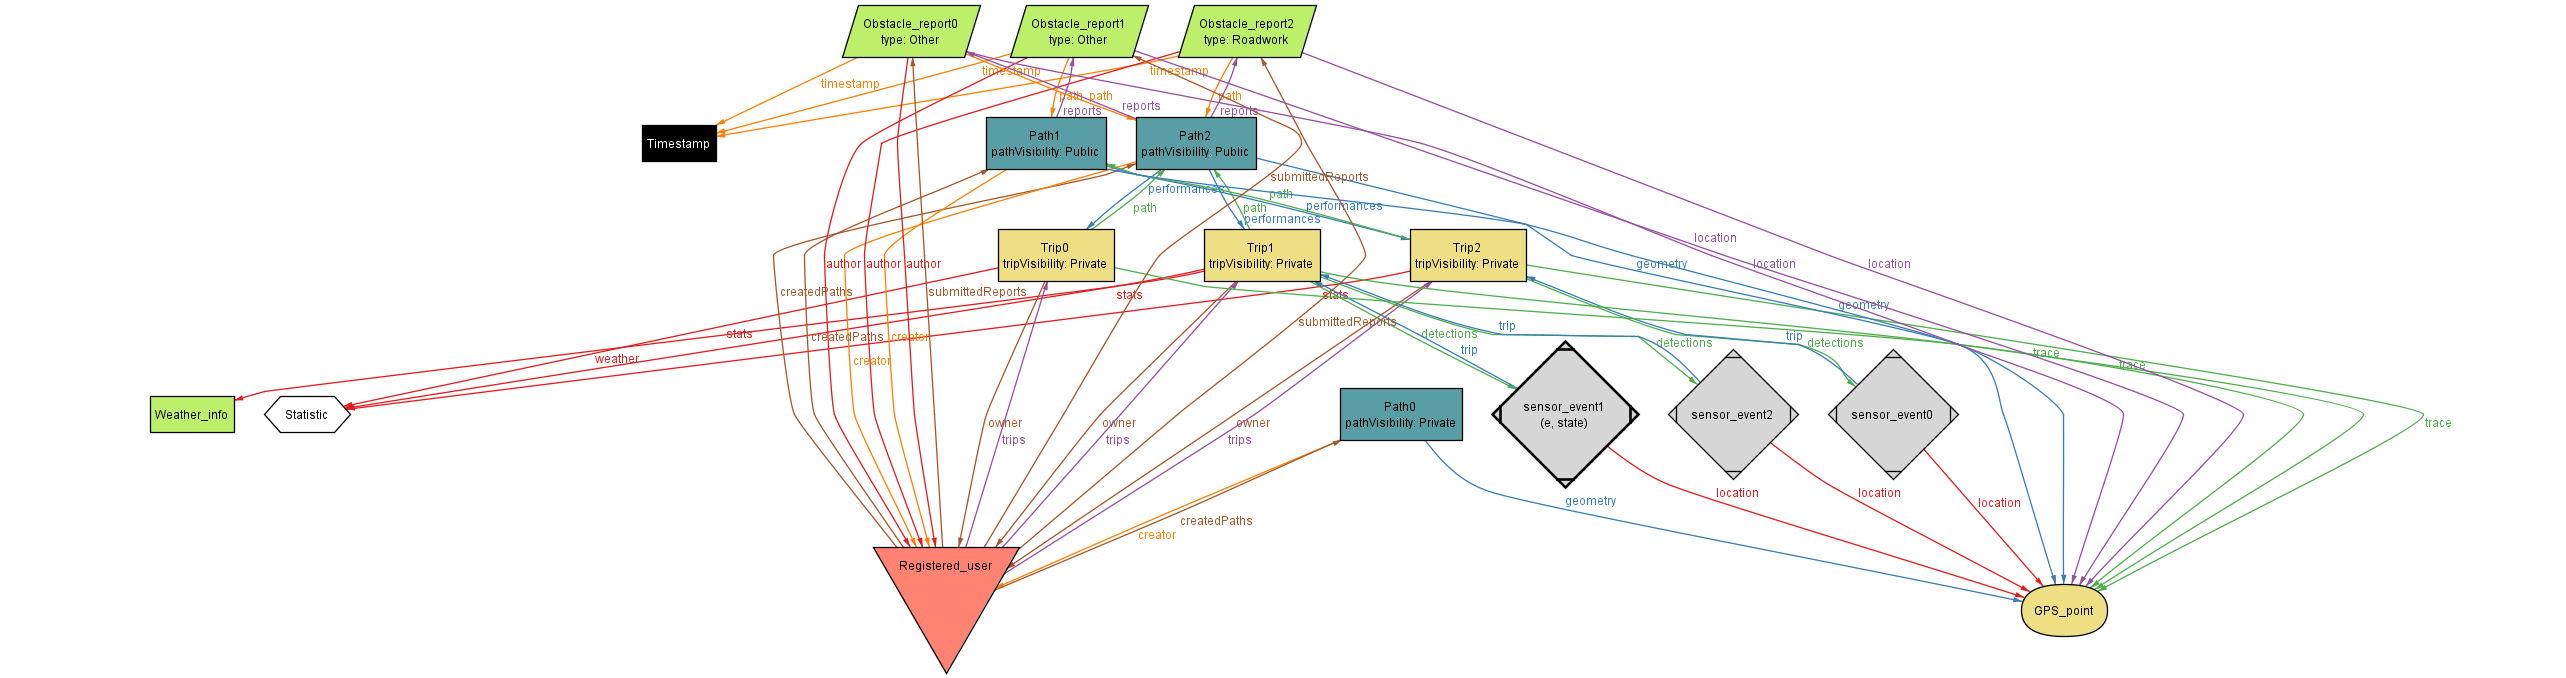
\includegraphics[width=1\linewidth]{RASD/LaTeXCode/Alloy/State 1 Projected View.png}
        \caption{State 1 Projected View}
        \label{fig:State 1 Projected View}%
    \end{center}
\end{figure}

\subsection{States 2}

\begin{figure}[H]
    \begin{center}
        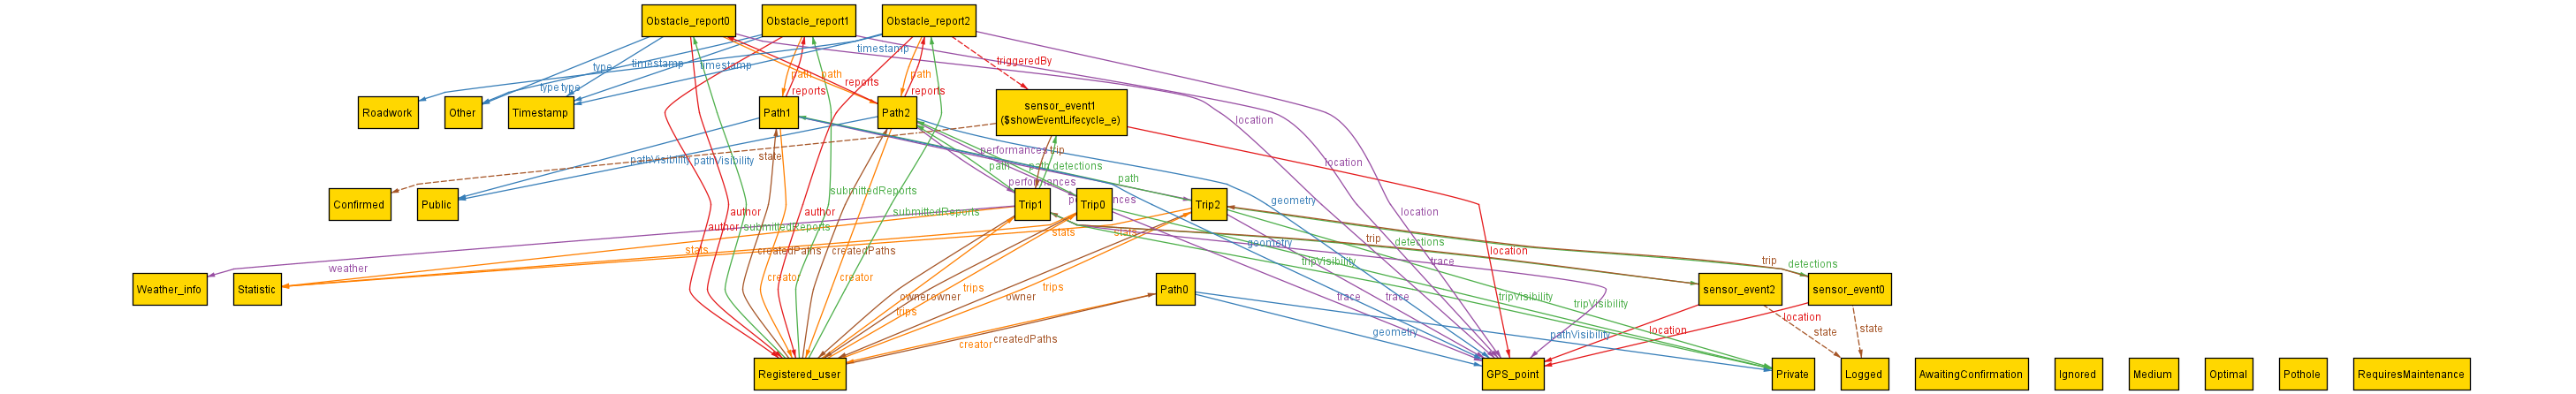
\includegraphics[angle=90,width=0.25\linewidth]{RASD/LaTeXCode/Alloy/State 2 Relational Graph.png}
        \caption{State 2 Relational Graph.}
        \label{fig:State 2 Relational Graph}%
    \end{center}
\end{figure}

\begin{figure}[H]
    \begin{center}
        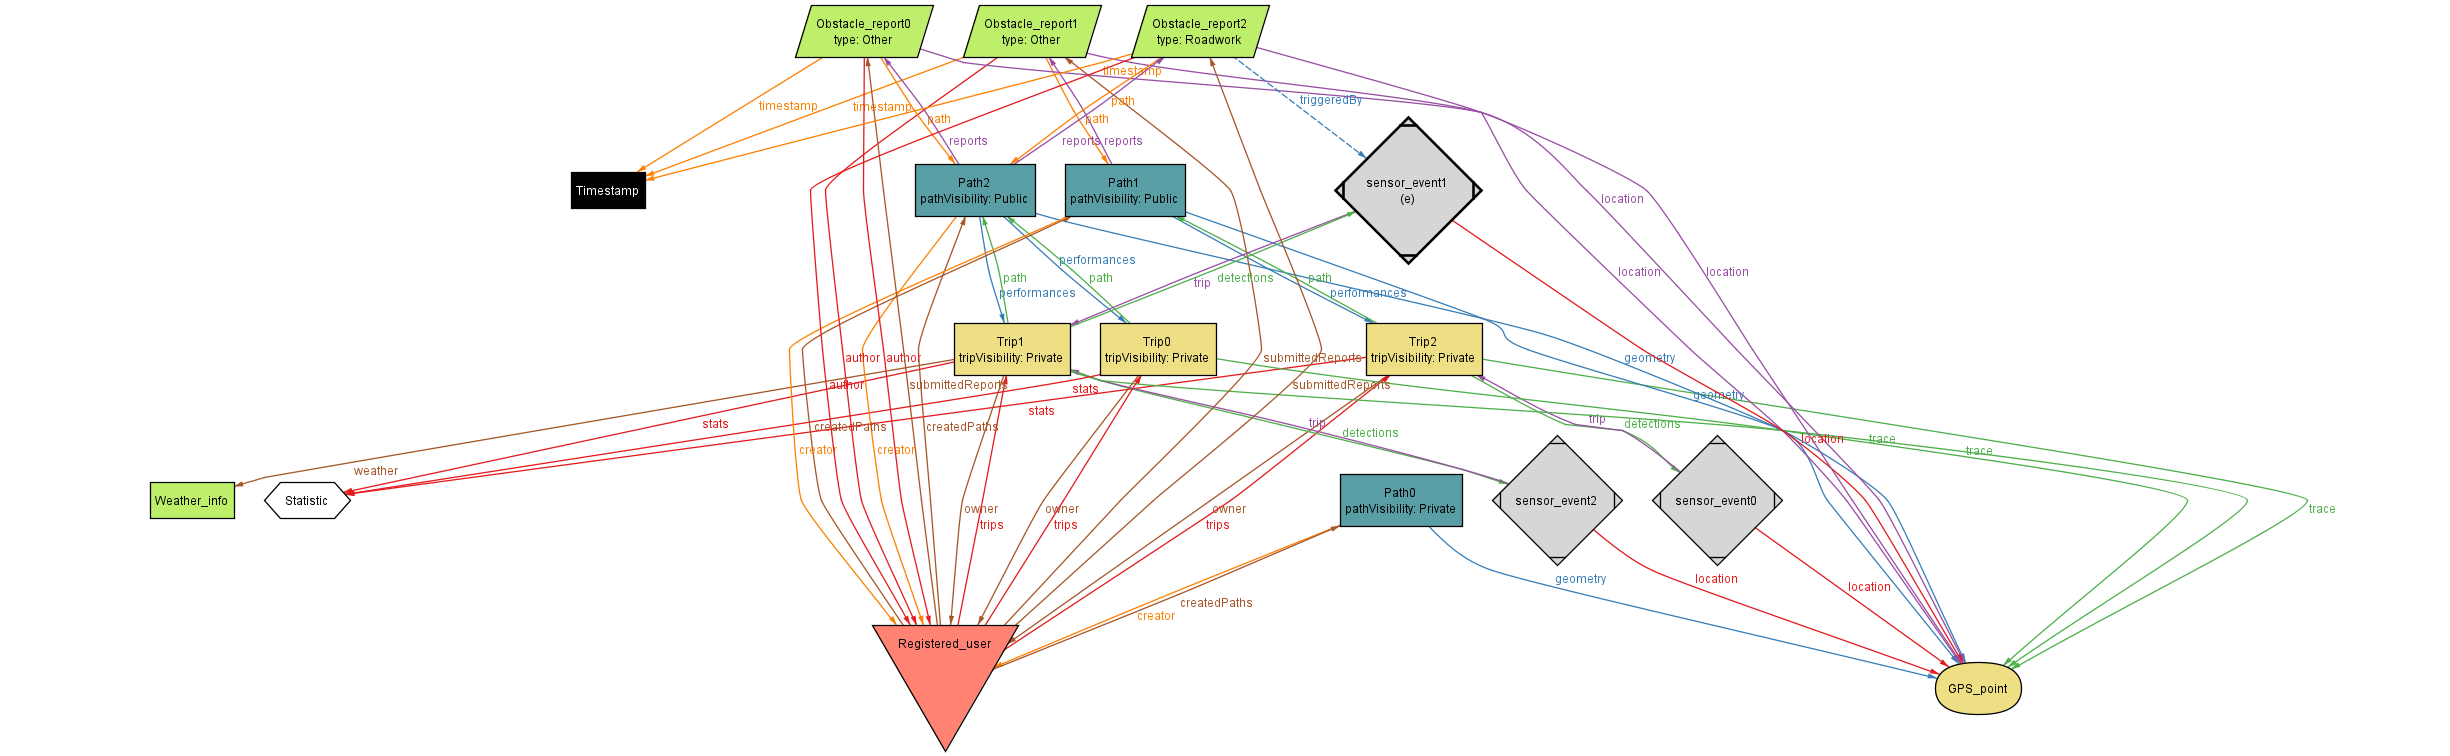
\includegraphics[width=1\linewidth]{RASD/LaTeXCode/Alloy/State 2 Projected View.png}
        \caption{State 2 Projected View}
        \label{fig:State 2 Projected View}%
    \end{center}
\end{figure}